\documentclass{beamer}

\usetheme[progressbar=frametitle]{metropolis}
\usepackage{appendixnumberbeamer}
\usepackage{booktabs}
\usepackage{amsmath}
\usepackage{amssymb}
\usepackage{tcolorbox}
\usepackage{tikz}

\definecolor{metropolisblue}{RGB}{39, 59, 94}



% Begin document
\begin{document}

% Title page
\title{Sampling Methods}
\author{Nipun Batra}
\date{\today}
\institute{IIT Gandhinagar}
\maketitle

\begin{frame}{Topics}
    %TOC with enumerated items
    \setbeamertemplate{section in toc}[sections numbered]
    \tableofcontents

\end{frame}


    \begin{frame}
        \href{https://www.youtube.com/watch?v=gMlf1ELvRzc}{The Discovery That Transformed Pi}
    \end{frame}

\begin{section}{Monte Carlo Simulation}
    \subsection{General Form}
    \begin{comment}
    \begin{frame}{The idea behind MC Simulation}
        \begin{itemize}
            \item We often want to compute expected value of some function of a random variable, which turns into the integral, 
            $$\mathbb{E} \left[ f (x) \right] = \int f(x) p(x) dx$$
            where $x \in \mathbb{R}^n, f: \mathbb{R}^n \rightarrow \mathbb{R}^m$ and $p(x)$ is the target distribution.
            \item In low dimensions, we can use numerical integration techniques to compute the above integral. However, in high dimensions, this is not feasible.
            \item Alternative approach is to draw  multiple random samples, $x_i \sim p(x)$ and compute
            $$\mathbb{E} \left[ f (x) \right] \approx \frac{1}{N} \sum_{i=1}^{N} f(x_i)$$
        \end{itemize}
    \end{frame}
\end{comment}

    \begin{frame}{General Form}

        The general form of Monte Carlo methods is:
        The expectation of a function $f(x)$ with respect to a distribution $p(x)$ is given by:
        \pause \begin{equation}
            % Expectation of f(x) with respect to p(x)
            \mathbb{E}_{x \sim p(x)}[f(x)] = \int f(x) p(x) dx
        \end{equation}
        
        \pause Using Monte Carlo methods, we can estimate the above expectation by sampling $x_i$ from $p(x)$ and computing the average of $f(x_i)$.
        \pause \begin{equation}
            % Monte Carlo estimate of expectation of f(x) with respect to p(x)
            \mathbb{E}_{x \sim p(x)}[f(x)] \approx \frac{1}{N} \sum_{i=1}^{N} f(x_i)
        \end{equation}
        where $x_i \sim p(x)$.

    \end{frame}

    % \begin{frame}{ }
    %     It is often difficult to compute the intergral $\int f(x) p(x) dx$ as it is expensive or intractable.
        
    %     Using Monte Carlo methods, we can estimate by sampling $x_i$ from $p(x)$ and computing the average of $f(x_i)$.
    %     \begin{equation}
    %         % Monte Carlo estimate of expectation of f(x) with respect to p(x)
    %         \mathbb{E}_{x \sim p(x)}[f(x)] \approx \frac{1}{N} \sum_{i=1}^{N} f(x_i)
    %     \end{equation}
    %     where $x_i \sim p(x)$.

    %     \begin{equation}
    %         % Expectation of f(x) with respect to p(x)
    %         \mathbb{E}_{x \sim p(x)}[f(x)] = \int f(x) p(x) dx
    %     \end{equation}
    %     Thus we can approximate the induced distribution, $p(x)$ sampling $x_i$ from $p(x)$ and computing the average of $f(x_i)$.
    % \end{frame}

    
    \subsection{Applications}
    \begin{frame}[fragile]{Estimating Pi using Monte Carlo (Part 1)}
        We can estimate the value of pi using Monte Carlo methods by considering a unit square with a quarter circle inscribed within it.
        
        \begin{itemize}
           \pause \item Let $p(x)$ be defined over the unit square using the uniform distribution in two dimensions, i.e., $p(x) = U(x) = 1$ for $x \in [0, 1]^2$.
            \pause \item Let $f(x)$ be the indicator function defined as follows:
                \[
                f(x) = \begin{cases}
                            \text{\textcolor{green}{Green}} (1), & \text{if } x \text{ falls inside the quarter circle}, \\
                            \text{\textcolor{red}{Red}} (0), & \text{otherwise}.
                       \end{cases}
                \]
        \end{itemize}
    \end{frame}

    \begin{frame}[fragile]{Estimating Pi using Monte Carlo (Part 1)}

        \begin{itemize}
        \item Or, we can write $f(x)$ to be the following:
            \[
            f(x) = \begin{cases}
                        1, & \text{if } x_1^2 + x_2^2 \leq 1, \\
                        0, & \text{otherwise}.
                   \end{cases}
            \]
        \item Or, using the indicator function, we can write $f(x)$ to be the following:
            \[
            f(x) = \mathbb{I}(x_1^2 + x_2^2 \leq 1)
            \]
        \end{itemize}
        
        \begin{center}
            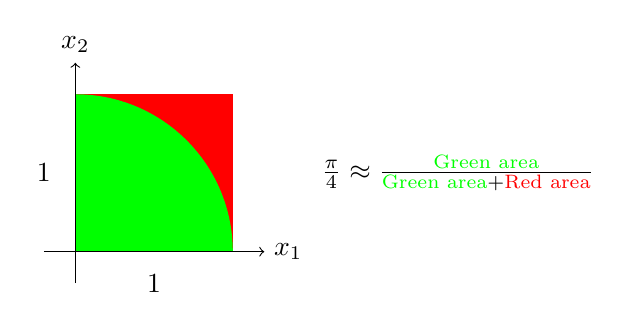
\begin{tikzpicture}[scale=2]
                % Unit Square
                \fill[red] (0,0) rectangle (1,1);
                
                % Quarter Circle
                \fill[green] (0,0) -- (0,1) arc (90:0:1) -- cycle;
                
                % Coordinate Axes
                \draw[->] (-0.2,0) -- (1.2,0) node[right] {$x_1$};
                \draw[->] (0,-0.2) -- (0,1.2) node[above] {$x_2$};
                
                % Labels
                \node at (0.5, -0.2) {1};
                \node at (-0.2, 0.5) {1};
                \node[right] at (1.5, 0.5) {$\frac{\pi}{4} \approx \frac{\text{\textcolor{green}{Green area}}}{\text{\textcolor{green}{Green area}} + \text{\textcolor{red}{Red area}}}$};
        
            \end{tikzpicture}
        \end{center}
    \end{frame}

    \begin{frame}
        Notebook: \url{mc_sampling_intro.ipynb}
    \end{frame}

    \begin{comment}

    \begin{frame}{Estimating a function using Monte Carlo}
        Let $x\in \mathcal{U}(-1,1)$ and $y = f(x) = x^2$.
        \begin{figure}
            \centering
        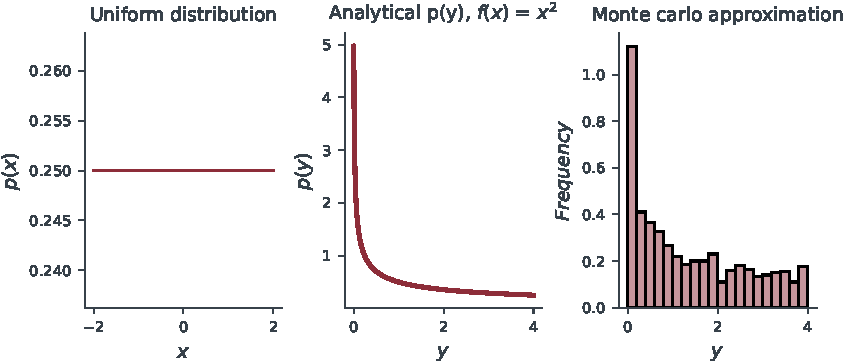
\includegraphics[scale=0.75]{../figures/mc_sampling_ex.pdf}
            \end{figure}    
    \end{frame}

\end{comment}

    \begin{frame}{Estimating prior predictive distribution}
        \begin{itemize}
            \item Let $p(\theta)$ be the prior distribution of parameter. Say, for example, $p(\theta_i) = \mathcal{N}(0, 1) ~\forall i$ or $p(\theta) = \mathcal{N}(\mu, \Sigma)$.
            \pause \item Let $p(y |\theta, x)$ be the likelihood function. Say, for example, $p(y|\theta, x) = \mathcal{N}(x^T\theta, 1)$.
            \pause \item Then, the prior predictive distribution is given by:
        \end{itemize}

            \begin{equation}
                p(y|x) = \int p(y|\theta, x) p(\theta) d\theta 
            \end{equation}

            \begin{equation}
                p(y|x) \approx \frac{1}{N} \sum_{i=1}^{N} p(y|\theta_i, x)
            \end{equation}
            where $\theta_i \sim p(\theta)$.
    \end{frame}

    \begin{frame}{Estimating prior predictive distribution}
        Notebook: \url{mc-linreg-predictive.ipynb}
    \end{frame}

    \begin{frame}{Estimating posterior predictive distribution}
        Extending for posterior predictive distribution, we have:

        \pause \begin{equation}
            p(y|x, D) = \int p(y|\theta, x) p(\theta|D) d\theta 
        \end{equation}

        \pause \begin{equation}
            p(y|x, D) \approx \frac{1}{N} \sum_{i=1}^{N} p(y|\theta_i, x)
        \end{equation}

        \pause where $\theta_i \sim p(\theta|D)$.
        
    \end{frame}

    \begin{frame}{Estimating marginal likelihood or evidence term for linear regression}
        [Ref: MML book 9.3.5]

        We consider the following generative process:
$$
\begin{aligned}
\boldsymbol{\theta} & \sim \mathcal{N}\left(\boldsymbol{m}_0, \boldsymbol{S}_0\right) \\
y_n \mid \boldsymbol{x}_n, \boldsymbol{\theta} & \sim \mathcal{N}\left(\boldsymbol{x}_n^{\top} \boldsymbol{\theta}, \sigma^2\right),
\end{aligned}
$$
$n=1, \ldots, N$. 

\pause The marginal likelihood is given by
$$
\begin{aligned}
p(\mathcal{Y} \mid \mathcal{X}) & =\int p(\mathcal{Y} \mid \mathcal{X}, \boldsymbol{\theta}) p(\boldsymbol{\theta}) \mathrm{d} \boldsymbol{\theta} \\
& =\int \mathcal{N}\left(\boldsymbol{y} \mid \boldsymbol{X} \boldsymbol{\theta}, \sigma^2 \boldsymbol{I}\right) \mathcal{N}\left(\boldsymbol{\theta} \mid \boldsymbol{m}_0, \boldsymbol{S}_0\right) \mathrm{d} \boldsymbol{\theta}
\end{aligned}
$$

\pause \begin{equation}
    =\mathcal{N}\left(\boldsymbol{y} \mid \boldsymbol{X} \boldsymbol{m}_0, \boldsymbol{X} \boldsymbol{S}_0 \boldsymbol{X}^{\top}+\sigma^2 \boldsymbol{I}\right)
    \end{equation}
        
    \end{frame}

    \begin{frame}{Estimating marginal likelihood or evidence term for linear regression}
        Instead if we used Monte Carlo methods, we would have:
        \pause \begin{equation}
            I = p(\mathcal{Y} \mid \mathcal{X}) \approx \frac{1}{N} \sum_{i=1}^{N} p(\mathcal{Y} \mid \mathcal{X}, \boldsymbol{\theta}_i)
        \end{equation}
        where $\boldsymbol{\theta}_i \sim p(\boldsymbol{\theta})$.
    \end{frame}
        
        \begin{frame}{Estimating Marginal Likelihood in Linear Regression}
            Generally, we work with log probabilities instead:
            
            \begin{equation}
                \log I = \log p(\mathcal{Y} \mid \mathcal{X}) \approx \log\left(\frac{1}{N} \sum_{i=1}^{N} p(\mathcal{Y} \mid \mathcal{X}, \boldsymbol{\theta}_i)\right)
            \end{equation}
            
            The log-sum-exp trick helps us compute this efficiently.
        \end{frame}
        

        \begin{frame}{Log-Sum-Exp Trick}
            [Ref: \url{https://gregorygundersen.com/blog/2020/02/09/log-sum-exp/}]

            The log-sum-exp trick is a technique to compute $\log\left(\frac{1}{N} \sum_{i=1}^{N} e^{a_i}\right)$ more efficiently.
            
            \begin{equation}
                \log\left(\frac{1}{N} \sum_{i=1}^{N} e^{a_i}\right) = \log\left(e^{\text{max}(a_i)} \frac{1}{N} \sum_{i=1}^{N} e^{a_i - \text{max}(a_i)}\right)
            \end{equation}
            
            \pause
            \begin{equation}
                = \text{max}(a_i) + \log\left(\frac{1}{N} \sum_{i=1}^{N} e^{a_i - \text{max}(a_i)}\right)
            \end{equation}
        \end{frame}
        
        \begin{frame}{Log-Sum-Exp Trick in Linear Regression}
            Applying the log-sum-exp trick to linear regression:
            
            \begin{equation}
                \log I = \log p(\mathcal{Y} \mid \mathcal{X}) \approx \log\left(\frac{1}{N} \sum_{i=1}^{N} p(\mathcal{Y} \mid \mathcal{X}, \boldsymbol{\theta}_i)\right)
            \end{equation}
            
            \begin{equation}
                = \log\left(\frac{1}{N} \sum_{i=1}^{N} e^{\log p(\mathcal{Y} \mid \mathcal{X}, \boldsymbol{\theta}_i)}\right)
            \end{equation}
            
            \pause
            \begin{equation}
                = \log\left(\frac{1}{N} \sum_{i=1}^{N} e^{\log p(\mathcal{Y} \mid \mathcal{X}, \boldsymbol{\theta}_i) - \text{max}(\log p(\mathcal{Y} \mid \mathcal{X}, \boldsymbol{\theta}_i))}\right)
            \end{equation}
            
            \pause
            \begin{equation}
                = \text{max}(\log p(\mathcal{Y} \mid \mathcal{X}, \boldsymbol{\theta}_i)) + \log\left(\frac{1}{N} \sum_{i=1}^{N} e^{\log p(\mathcal{Y} \mid \mathcal{X}, \boldsymbol{\theta}_i) - \text{max}(\log p(\mathcal{Y} \mid \mathcal{X}, \boldsymbol{\theta}_i))}\right)
            \end{equation}
        \end{frame}
        
        \begin{frame}{Efficient Computation}
            The log-sum-exp trick allows us to compute $\log I$ more efficiently by:
            
            \begin{itemize}
                \item Subtracting the maximum value of $\log p(\mathcal{Y} \mid \mathcal{X}, \boldsymbol{\theta}_i)$ to avoid numerical issues with exponentiation.
                \item Adding the maximum value back after the sum of exponentials.
            \end{itemize}
            
            This technique helps prevent overflow and underflow issues when dealing with large or small values in the exponentials.
        \end{frame}


        \begin{frame}{Estimating Marginal Likelihood in Linear Regression}
            Notebook: \url{mc-linreg-evidence.ipynb}
            
        \end{frame}
        

 


    \subsection{Bias and Variance of Monte Carlo}
    \begin{frame}{Unbiased Estimator?}
        Is Monte Carlo Sampling a biased or unbiased estimator?

        We know:
        \begin{equation}
            % Expectation of f(x) with respect to p(x)
            \mathbb{E}_{x \sim p(x)}[f(x)] = \int f(x) p(x) dx = \phi
        \end{equation}
        Let $x_i\in 1, \ldots, N$ be i.i.d samples:
        \begin{align*}
            \hat{\phi} &= \frac{1}{N} \sum_{i=1}^{N} f(x_i) \\
            \mathbb{E}(\hat{\phi}) &= \int \frac{1}{N} \sum_{i=1}^{N} f(x_i)p(x_i)dx = \frac{1}{N}\sum_{i=1}^{N} \int f(x_i)p(x_i)dx \\
            &= \frac{1}{N}\sum_{i=1}^N\mathbb{E}(f(x_i)) = \phi
        \end{align*}
        Thus, it is an unbiased estimator!
    \end{frame}

    \begin{frame}{Sampling converges slowly}
        The expected square error of the Monte Carlo estimate is given by:
        $$
        \mathbb{E} \left( \hat{\phi} - \mathbb{E} (\hat{\phi}) \right)^2 = \mathbb{E} \left[ \frac{1}{N} \sum_{i=1}^{N} (f(x_i) - \phi) \right]^2 
        $$
        $$
        = \frac{1}{N^2} \sum_{i=1}^{N} \sum_{j=1}^{N} \mathbb{E} (f(x_i) f(x_j)) - \phi \mathbb{E} (f(x_i)) - \mathbb{E} (f(x_j)) \phi + \phi^2
        $$
        $$
        = \frac{1}{N^2} \sum_{i=1}^{N} \left( \left( \sum_{i \neq j}^{} \phi^2 - 2 \phi^2 + \phi^2 \right) + \mathbb{E} (f^2) - \phi^2 \right) = \frac{1}{N} \mathbb{V} (f)
        $$
        $$
        \therefore \mathbb{E} \left( \hat{\phi} - \mathbb{E} (\hat{\phi}) \right)^2 = \mathcal{O} (N^{-1})
        $$
        Thus, the expected error drops as $\mathcal{O} (N^{-\frac{1}{2}})$.
    \end{frame}

    \begin{comment}
    \begin{frame}{Pop Quiz}
        How many samples ($N$) do we need to reach single-precision (i.e., $\sim 10^{-7}$)?
    \end{frame}

    \begin{frame}{Is sampling easy?}
        Many reasons contribute to sampling not always being easy in higher dimensions. For example,
        \begin{itemize}
            \item need a global description of the entire function
            \item need to know probability densities everywhere
            \item need to know regions of high density
        \end{itemize}
    \end{frame}
\end{comment}
    
\end{section}


\begin{section}{Sampling from common probability distributions}
    \begin{subsection}{PRNG}

    \begin{frame}{Sampling from uniform U(0, 1)}
        [Ref: \url{https://en.wikipedia.org/wiki/Linear_congruential_generator}]
        
    
    \begin{itemize}
        \item Question: How can you generate samples from the uniform distribution in $[0, 1]$?
        \item \pause Hint: Linear Congruential Generator (LCG) among other PRNGs.
        \item \pause \begin{equation}
            x_{n+1} = (a x_n + c) \mod m
        \end{equation}
        \item  where, $a, c, m$ are constants and $x_0$ is the seed
        \item $x_{n+1}$ is the next random number between 0 and $m-1$
        \item \pause $\frac{x_{n+1}}{m}$ is the next random number between 0 and 1
    

    \end{itemize}
\end{frame}

\begin{frame}{Sampling from uniform U(0, 1)}
    From Wikipedia page on LCG

    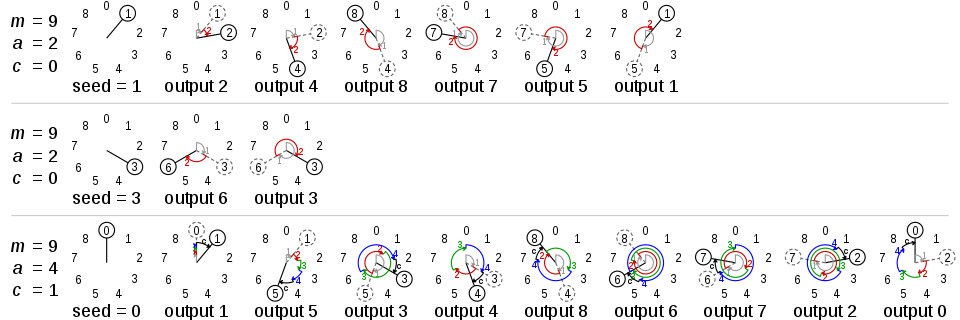
\includegraphics[width=\columnwidth]{../figures/wiki-LCG.png}
    
\end{frame}

\begin{frame}{Sampling from uniform U(0, 1)}
Notebook: random-uniform.ipynb
    
\end{frame}

\begin{frame}{Sampling from uniform U(a, b)}
    \begin{itemize}
        \item Assume we have $X \sim U(0, 1)$
        \item \pause Then, $Y = a + (b - a) X \sim U(a, b)$
    \end{itemize}
    
\end{frame}

\end{subsection}

\subsection{Inverse CDF Sampling}
\begin{frame}{Inverse CDF sampling}
    [Inspired by content from Ben Lambert and Phillip Hennig]
    \begin{itemize}
        \item Let us try to generate samples from the exponential distribution. 
        \item \pause The PDF of the exponential distribution is given by:
        \item \pause PDF: $p(x) = \lambda e^{-\lambda x}$
        \item \pause CDF: $F(x) = 1 - e^{-\lambda x}$. Prove!
        
    \end{itemize}

    \begin{figure}
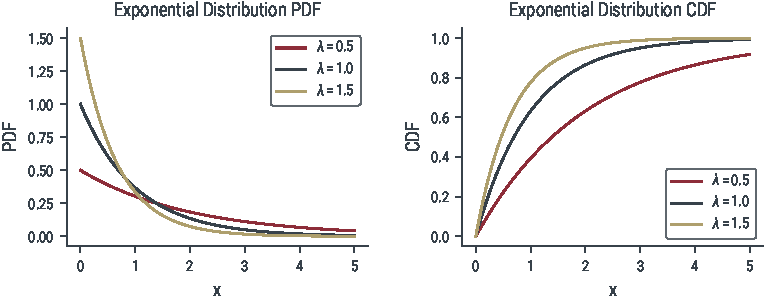
\includegraphics[width=\columnwidth]{../figures/sampling/exp-cdf.pdf}
    \end{figure}
    
\end{frame}

\subsection{Inverse CDF Sampling}
\begin{frame}{Inverse CDF sampling}
    \begin{itemize}
        \item \pause PDF: $p(x) = \lambda e^{-\lambda x}$
        \item \pause CDF: $F(x) = 1 - e^{-\lambda x}$. Prove!
        
    \end{itemize}

    \begin{equation}
        F(x) = \int_{-\infty}^{x} p(x) dx
    \end{equation}

    \begin{equation}
        F(x) = \int_{-\infty}^{x} \lambda e^{-\lambda x} dx
    \end{equation}


    \begin{equation}
        F(x) = \left[ -e^{-\lambda x} \right]_{-\infty}^{x}
    \end{equation}

    \begin{equation}
        F(x) = 1 - e^{-\lambda x}
    \end{equation}

    
\end{frame}



% Loop for lambda values from 1 to 10
\foreach \ns in {1,2,3,4,5,6,7,8,9}{
  \begin{frame}{Inverse CDF Sampling for Number of samples = \ns}
    \begin{itemize}
        \item Let us consider the CDF ($F(x)$) of the exponential distribution ($\lambda=1$) and try to generate samples from it.
        \item We generate a random number $u \sim U(0, 1)$.
        \item We then find the value of $x$ such that $F(x) = u$.
    \end{itemize}
  
    \begin{figure}
        \includegraphics[width=0.7\textwidth]{../figures/sampling/exp-cdf-samples-\ns.pdf}
    \end{figure}
  \end{frame}
}


       
   \begin{frame}{Inverse CDF sampling}


        \begin{itemize}
    
            \item We generate a random number $u \sim U(0, 1)$.
            \item \pause We then find the value of $x$ such that $F(x) = u$.
    \item \pause This is equivalent to finding the inverse of the CDF, i.e., $F^{-1}(u)$.
        \item \pause For the exponential distribution, let us try to find $F^{-1}(u)$.
        \item \pause  $u = 1 - e^{-x}$
        
        \item \pause 
            $x = -\log(1 - u)$
        
    \end{itemize}
        
    
\end{frame}

\begin{frame}
    Notebook: inverse-cdf.ipynb
\end{frame}

\begin{frame}{Inverse CDF sampling}
    [From Wikipedia page on Inverse Transform Sampling]

    \url{https://en.wikipedia.org/wiki/Inverse_transform_sampling}

\end{frame}

\subsection{Sampling from Normal Distribution}
\begin{frame}{Generating samples from $\mathcal{N}(0, 1)$ using Box-Muller Transform}
    [From Wikipedia page on Box-Muller Transform]
    \begin{itemize}
        \item Let $U_1, U_2 \sim U(0, 1)$ be two independent random variables.
        \item \pause Let $Z_0, Z_1 \sim \mathcal{N}(0, 1)$ be two independent random variables.
        \item \pause Then, $R = \sqrt{-2 \log U_1}$ and $\Theta = 2 \pi U_2$ are independent random variables.
        \item \pause Then, $Z_0 = R \cos \Theta$ and $Z_1 = R \sin \Theta$ are independent random variables.
        \item \pause $Z_0$ and $Z_1$ are independent and identically distributed (i.i.d) $\mathcal{N}(0, 1)$ random variables.
    \end{itemize}
    
\end{frame}

\begin{frame}
    Notebook: sampling-normal.ipynb
\end{frame}

\begin{frame}{Generating samples from $\mathcal{N}(\mu, \sigma)$}
    \begin{itemize}
        \item Let $Z_0 \sim \mathcal{N}(0, 1)$ be independent random variables.
        \item \pause Then, $X = \mu + \sigma Z_0$ is a random variable with $\mathcal{N}(\mu, \sigma)$ distribution.
    \end{itemize}
    
\end{frame}

\begin{frame}{Generating samples from Multivariate $\mathcal{N}(\mu, \Sigma)$}
    Drawing values from the distribution in \url{https://en.wikipedia.org/wiki/Multivariate_normal_distribution}
\end{frame}


    
\end{section}

\subsection{Rejection Sampling}
    \begin{frame}{Rejection Sampling}
        \begin{itemize}
            \item Let $p(x)$ be the target distribution from which we want to sample.
            \pause \item Let $q(x)$ be a proposal distribution from which we can sample.
            \pause \item Let $M$ be a constant such that $M \geq \frac{p(x)}{q(x)} \forall x$.
            \pause \item Then, we can sample from $p(x)$ by sampling from $q(x)$ and accepting the sample with probability $\frac{p(x)}{M q(x)}$.
        \end{itemize}
        
    \end{frame}

    \begin{frame}
        Notebook: \url{rejection-sampling.ipynb}
    \end{frame}

   \begin{frame}{Rejection Sampling}
    \begin{figure}
        \centering
        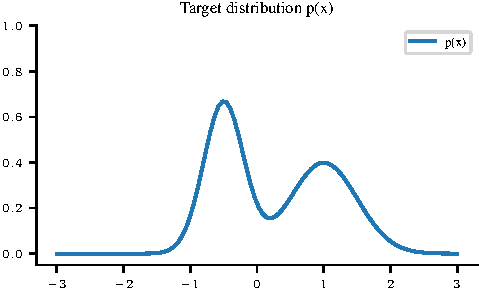
\includegraphics[scale = 0.75]{../figures/sampling/rejection-sampling--1.0-False-False-False-False-False-False-False-False.pdf}
    \end{figure}
    
   \end{frame}

    \begin{frame}{Rejection Sampling}
        \begin{figure}
            \centering
            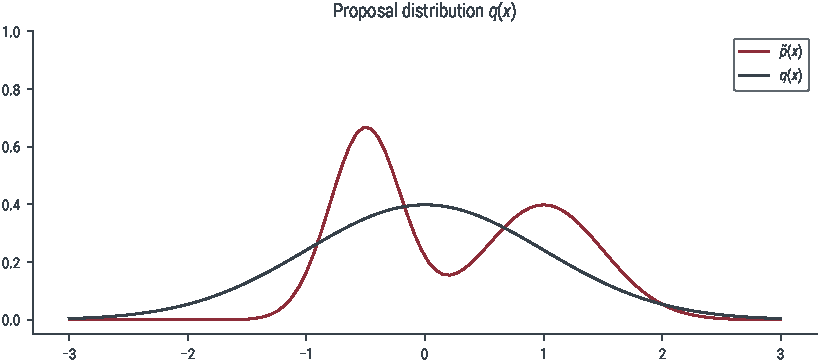
\includegraphics[scale = 0.75]{../figures/sampling/rejection-sampling--1.0-True-False-False-False-False-False-False-False.pdf}
        \end{figure}
    \end{frame}

    \begin{frame}{Rejection Sampling}
        \begin{figure}
            \centering
            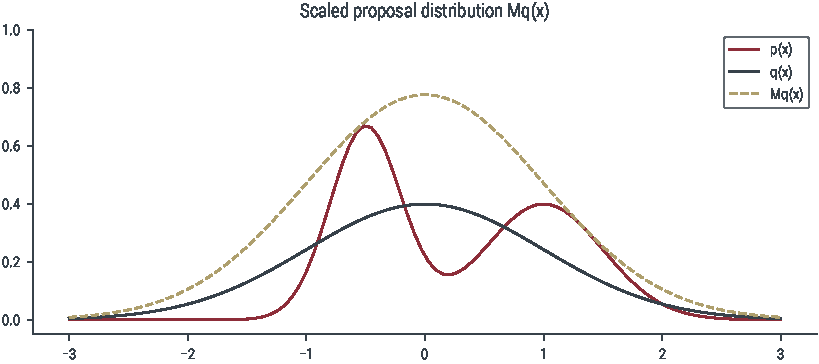
\includegraphics[scale = 0.75]{../figures/sampling/rejection-sampling--1.0-True-True-False-False-False-False-False-False.pdf}
        \end{figure}
    \end{frame}

    \begin{frame}{Rejection Sampling}
        \begin{figure}
            \centering
            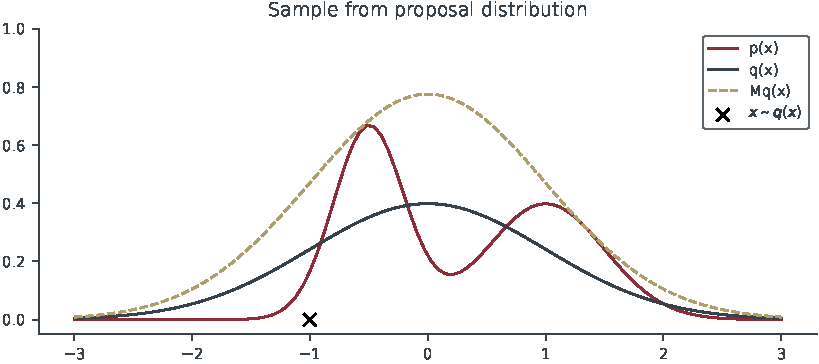
\includegraphics[scale = 0.75]{../figures/sampling/rejection-sampling--1.0-True-True-True-False-False-False-False-False.pdf}
        \end{figure}
    \end{frame}

    \begin{frame}{Rejection Sampling}
        \begin{figure}
            \centering
            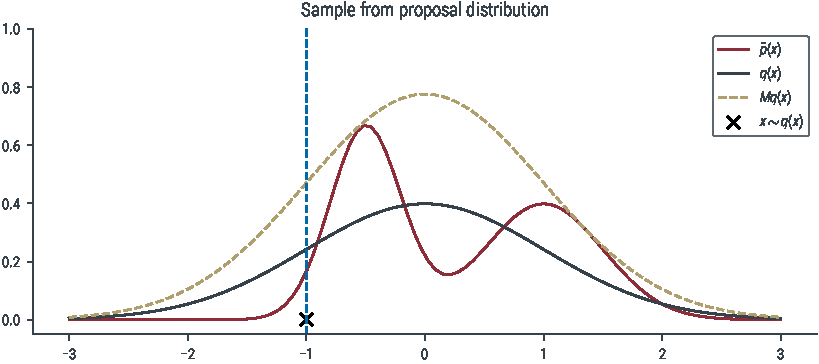
\includegraphics[scale = 0.75]{../figures/sampling/rejection-sampling--1.0-True-True-True-True-False-False-False-False.pdf}
        \end{figure}
    \end{frame}

    \begin{frame}{Rejection Sampling}
        \begin{figure}
            \centering
            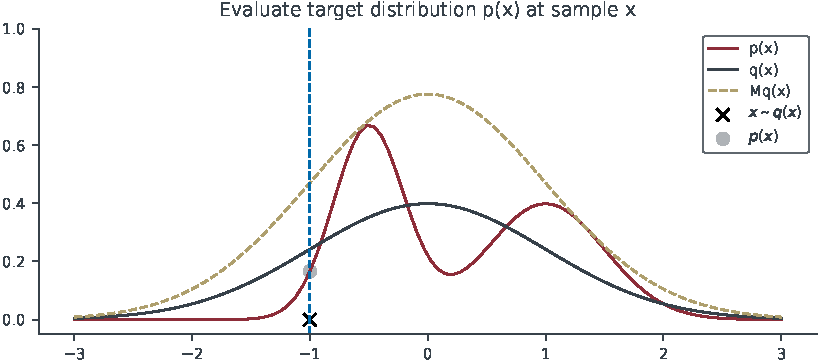
\includegraphics[scale = 0.75]{../figures/sampling/rejection-sampling--1.0-True-True-True-True-True-False-False-False.pdf}
        \end{figure}
    \end{frame}

    \begin{frame}{Rejection Sampling}
        \begin{figure}
            \centering
            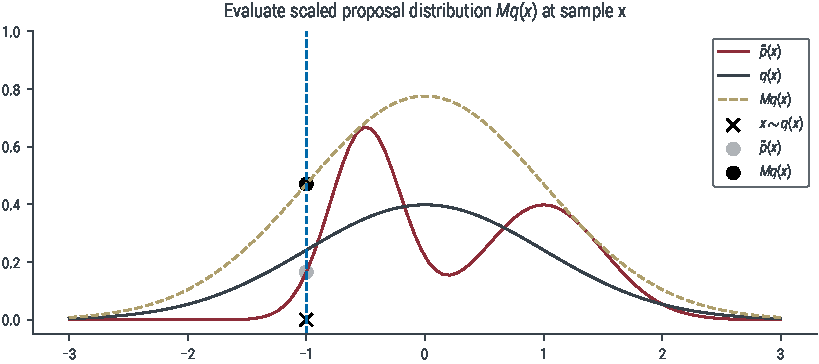
\includegraphics[scale = 0.75]{../figures/sampling/rejection-sampling--1.0-True-True-True-True-True-True-False-False.pdf}
        \end{figure}
    \end{frame}

    \begin{frame}{Rejection Sampling}
        \begin{figure}
            \centering
            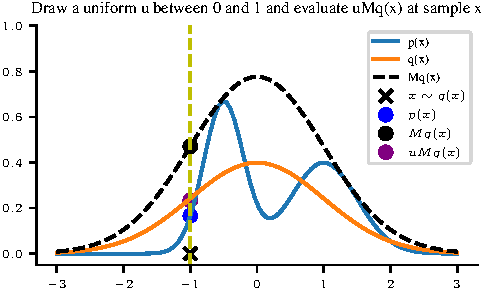
\includegraphics[scale = 0.75]{../figures/sampling/rejection-sampling--1.0-True-True-True-True-True-True-True-False.pdf}
        \end{figure}
    \end{frame}

    \begin{frame}{Rejection Sampling (Rejected Sample)}
        \begin{figure}
            \centering
            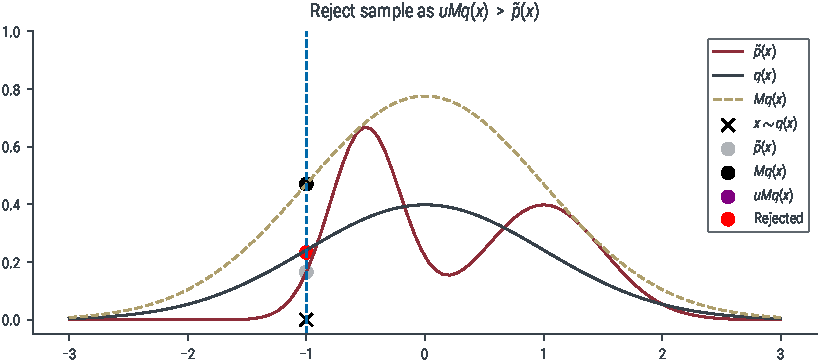
\includegraphics[scale = 0.75]{../figures/sampling/rejection-sampling--1.0-True-True-True-True-True-True-True-True.pdf}
        \end{figure}
    \end{frame}


    \begin{frame}{Rejection Sampling (Accepted Sample)}
        \begin{figure}
            \centering
            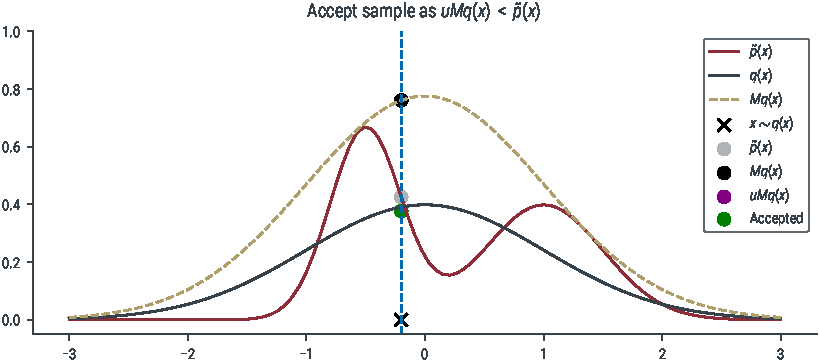
\includegraphics[scale = 0.75]{../figures/sampling/rejection-sampling--0.2-True-True-True-True-True-True-True-True.pdf}
        \end{figure}
    \end{frame}

    \foreach \n in {10, 1000, 10000}{
    \begin{frame}{Rejection Sampling (\n{} samples)}
        \includegraphics[width=\textwidth]{../figures/sampling/rejection-sampling-N\n-False.pdf}
    \end{frame}

    \begin{frame}{Rejection Sampling (\n{} samples) (KDE)}
        \includegraphics[width=\textwidth]{../figures/sampling/rejection-sampling-N\n-True.pdf}
    \end{frame}
}

   
    \begin{frame}{Proof of Rejection Sampling}
        \begin{tcolorbox}[colback=metropolisblue!5,colframe=metropolisblue,title={Acceptance Probability $\alpha(x)$}]
            \begin{equation}
              \alpha(x) = \frac{p(x)}{M q(x)}
            \end{equation}
        \end{tcolorbox}
       
        \begin{tcolorbox}[colback=metropolisblue!5,colframe=metropolisblue,title={Bayes Rule for Acceptance}]
            \begin{equation}
                P(Sample|Accept) = \frac{P(Accept|Sample) P(Sample)}{P(Accept)}
            \end{equation}
        \end{tcolorbox}

        \begin{tcolorbox}[colback=metropolisblue!5,colframe=metropolisblue,title={P(Sample)}]
            We draw samples from $q(x)$, so $P(Sample) = q(x)$.
        \end{tcolorbox}
    \end{frame}

    \begin{frame}{Proof of Rejection Sampling}

        Further, $P(Accept|Sample) = \alpha(x) = \dfrac{p(x)}{M q(x)}$.

        Finally, $P(Accept) = \int P(Accept|Sample) P(Sample) dSample = \int \alpha(x) q(x) dx = \dfrac{1}{M} \int p(x) dx = \dfrac{1}{M}$.
        \begin{tcolorbox}[colback=metropolisblue!5,colframe=metropolisblue,title={P(Accept)}]
            \begin{equation}
                P(Accept) = \frac{1}{M}
            \end{equation}
        \end{tcolorbox}
        

        Thus, $P(Sample|Accept) = \dfrac{p(x)}{M q(x)} \times \dfrac{q(x)}{1/M} = p(x)$.

        Thus, we have shown that the samples we accept are distributed according to $p(x)$.
        
    \end{frame}

    \begin{frame}{Rejection Sampling Completed Example}
        Note: Figures not on github.
    \end{frame}

    % \begin{frame}{Rejection Sampling Completed Example}
    %     \begin{figure}
    %         \centering
    %         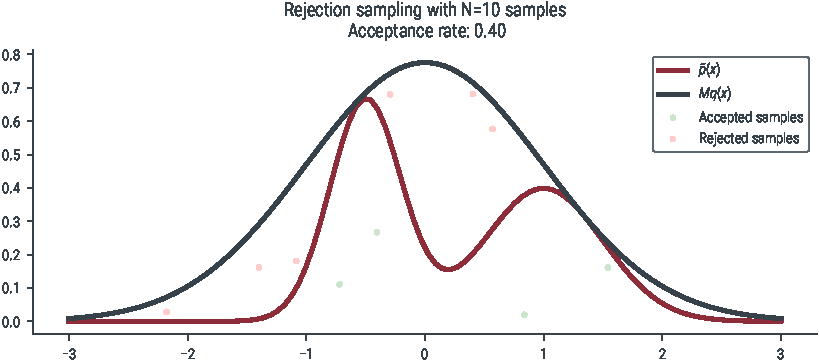
\includegraphics[scale = 0.75]{../figures/sampling/rejection-sampling-N10-False.pdf}
    %     \end{figure}
        
    % \end{frame}

    % \begin{frame}{Rejection Sampling Completed Example}
    %     \begin{figure}
    %         \centering
    %         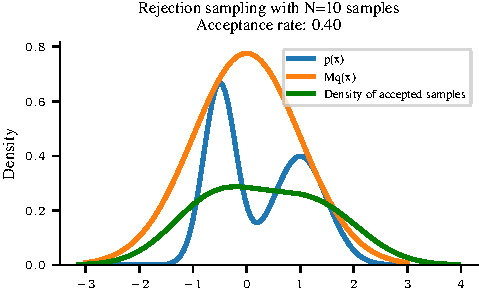
\includegraphics[scale = 0.75]{../figures/sampling/rejection-sampling-N10-True.pdf}
    %     \end{figure}
        
    % \end{frame}

    % \begin{frame}{Rejection Sampling Completed Example}
    %     \begin{figure}
    %         \centering
    %         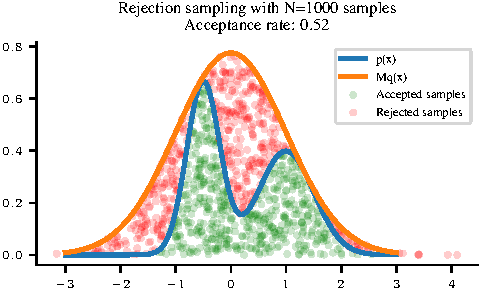
\includegraphics[scale = 0.75]{../figures/sampling/rejection-sampling-N1000-False.pdf}
    %     \end{figure}
    % \end{frame}

    % \begin{frame}{Rejection Sampling Completed Example}
    %     \begin{figure}
    %         \centering
    %         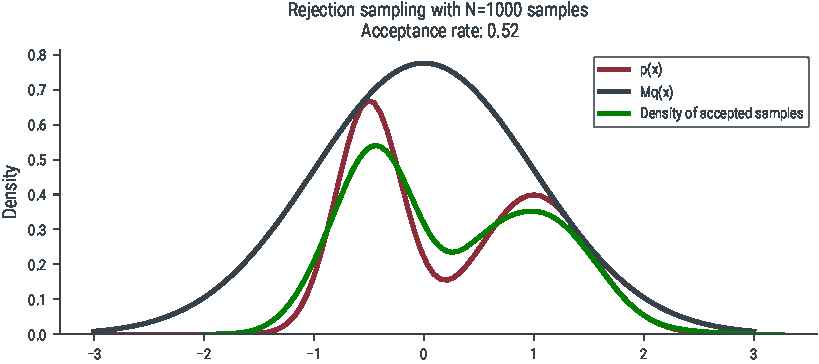
\includegraphics[scale = 0.75]{../figures/sampling/rejection-sampling-N1000-True.pdf}
    %     \end{figure}
    % \end{frame}

    % \begin{frame}{Rejection Sampling Completed Example}
    %     \begin{figure}
    %         \centering
    %         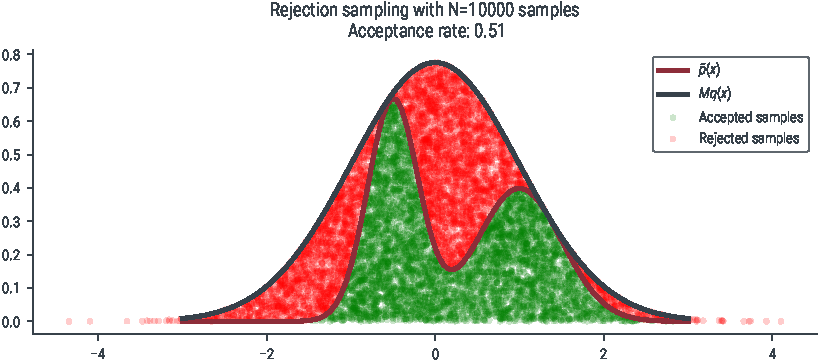
\includegraphics[scale = 0.75]{../figures/sampling/rejection-sampling-N10000-False.pdf}
    %     \end{figure}
    % \end{frame}

    % \begin{frame}{Rejection Sampling Completed Example}
    %     \begin{figure}
    %         \centering
    %         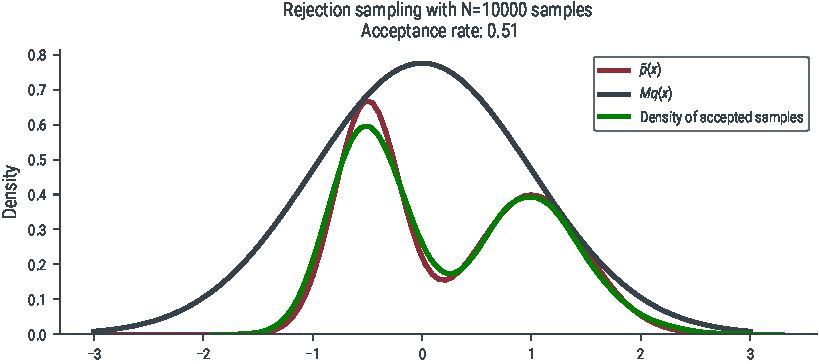
\includegraphics[scale = 0.75]{../figures/sampling/rejection-sampling-N10000-True.pdf}
    %     \end{figure}
    % \end{frame} 

    \begin{frame}{Challenges with Rejection Sampling}
        \begin{itemize}
            \item Rejection sampling is inefficient when the target distribution is very different from the proposal distribution.
            \item In this case, we will reject a lot of samples.
            \item This is a problem when sampling from high-dimensional distributions.
            \item Acceptance probability $\alpha(x)$ is very low.
        \end{itemize}
    \end{frame}




\end{document}